% This is samplepaper.tex, a sample chapter demonstrating the
% LLNCS macro package for Springer Computer Science proceedings;
% Version 2.21 of 2022/01/12
%
\documentclass[runningheads]{llncs}
%
\usepackage[brazil]{babel}
\usepackage[T1]{fontenc}
% T1 fonts will be used to generate the final print and online PDFs,
% so please use T1 fonts in your manuscript whenever possible.
% Other font encondings may result in incorrect characters.
%
\usepackage{hyperref}
\usepackage{graphicx}
% Used for displaying a sample figure. If possible, figure files should
% be included in EPS format.
%
% If you use the hyperref package, please uncomment the following two lines
% to display URLs in blue roman font according to Springer's eBook style:
\usepackage{color}
\renewcommand\UrlFont{\color{blue}\rmfamily}
\urlstyle{rm}
%
\begin{document}
%
\title{Predição de Problemas Cardíacos por Modelos de Classificação de Aprendizado de Máquina}
%
%\titlerunning{Abbreviated paper title}
% If the paper title is too long for the running head, you can set
% an abbreviated paper title here
%
\author{João Victor Lopez Pereira\inst{1,2} \and
Yuri Rocha de Albuquerque\inst{1,3}}
%
\authorrunning{Pereira, J.V.L., Albuquerque, Y.R..}
% First names are abbreviated in the running head.
% If there are more than two authors, 'et al.' is used.
%
\institute{Universidade Federal do Rio de Janeiro, Rio de Janeiro RJ, Brasil \\
\and
\email{joaovictorlopezpereira@gmail.com}\\
\and
\email{yurira@ic.ufrj.br}}
%
\maketitle              % typeset the header of the contribution
%
\begin{abstract}
The abstract should briefly summarize the contents of the paper in
150--250 words.

\keywords{First keyword  \and Second keyword \and Another keyword.}
\end{abstract}
%
%


% \begin{figure}
%   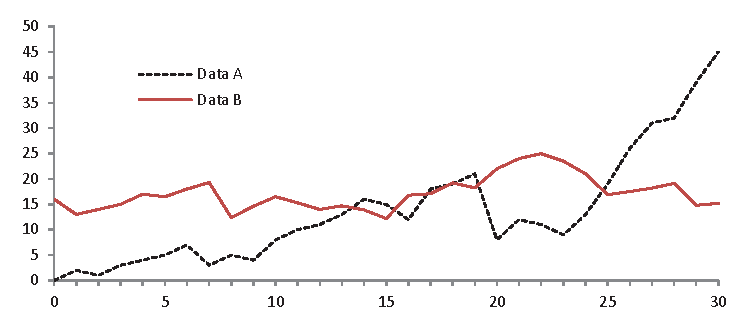
\includegraphics[width=\textwidth]{fig1.eps}
%   \caption{A figure caption is always placed below the illustration.
%   Please note that short captions are centered, while long ones are
%   justified by the macro package automatically.} \label{fig1}
% \end{figure}



% \begin{credits}
% \subsubsection{\discintname}
% It is now necessary to declare any competing interests or to specifically
% state that the authors have no competing interests. Please place the
% statement with a bold run-in heading in small font size beneath the
% (optional) acknowledgments\footnote{If EquinOCS, our proceedings submission
% system, is used, then the disclaimer can be provided directly in the system.},
% for example: The authors have no competing interests to declare that are
% relevant to the content of this article. Or: Author A has received research
% grants from Company W. Author B has received a speaker honorarium from
% Company X and owns stock in Company Y. Author C is a member of committee Z.
% \end{credits}
%
% ---- Bibliography ----
%
% BibTeX users should specify bibliography style 'splncs04'.
% References will then be sorted and formatted in the correct style.
%
% \bibliographystyle{splncs04}
% \bibliography{mybibliography}
%
\begin{thebibliography}{8}

\bibitem{fedesorianoheartfailure2021}
Fedesoriano:
Heart Failure Prediction Dataset.
\url{https://www.kaggle.com/datasets/fedesoriano/heart-failure-prediction},
last accessed 2025/11/11

\bibitem{PereiraAlbuquerque2025}
Pereira, J.V.L., Albuquerque, Y.R.:
Heart-Failure-Predictor: Machine learning project for heart failure prediction using clinical data.
\url{https://github.com/joaovictorlopezpereira/Heart-Failure-Predictor},
last accessed 2025/11/12

\end{thebibliography}

\end{document}
